\documentclass{article}

\usepackage[final]{neurips_2019}

\usepackage[utf8]{inputenc}
\usepackage[T1]{fontenc}
\usepackage{hyperref}
\usepackage{url}
\usepackage{booktabs}
\usepackage{amsfonts}
\usepackage{amsmath, bm, bbm}
\usepackage{amssymb}
\usepackage{nicefrac}
\usepackage{microtype}
\usepackage{graphicx}
\usepackage{xcolor}
\usepackage{lipsum}
\usepackage{makecell}

\newcommand{\note}[1]{\textcolor{blue}{{#1}}}

\title{
  Exploring CNNs in Question Answering \\
  \vspace{1em}
  \small{\normalfont Stanford CS224N Default Project}  % Select one and delete the other
}

\author{
  Joseph Pagadora, $\;$ Steve Gan \\
  Stanford University \\
  \texttt{jcp737@stanford.edu}$\;\;\;\;$
  \texttt{zgan@stanford.edu} \\
  % Examples of more authors
%   \And
%   Name \\
%   Department of Computer Science \\
%   Stanford University \\
%   \texttt{name@stanford.edu} \\
%   \And
%   Name \\
%   Department of Computer Science \\
%   Stanford University \\
%   \texttt{name@stanford.edu}
}

\begin{document}

\maketitle

% \begin{abstract}
%   Required for final report
% \end{abstract}

\begin{abstract}
The goal of this project is to reproduce the QANet model described in \cite{YU} and improve on this model. So far, we have focused on an implementation of QANet and BiDAF with character-level embedding in PyTorch. Unfortunately, as for now, we are not able to finish 30 epochs of training for either of the QANet model or BiDAF because of CUDA errors. We also plan to implement the data augmentation approach through backtranslation and explore improvement ideas such as changing span representation and tweaking the attention mechanism and the backtranslation pipeline.
\end{abstract}

\section{Approach}

\begin{figure}[h]
\centering
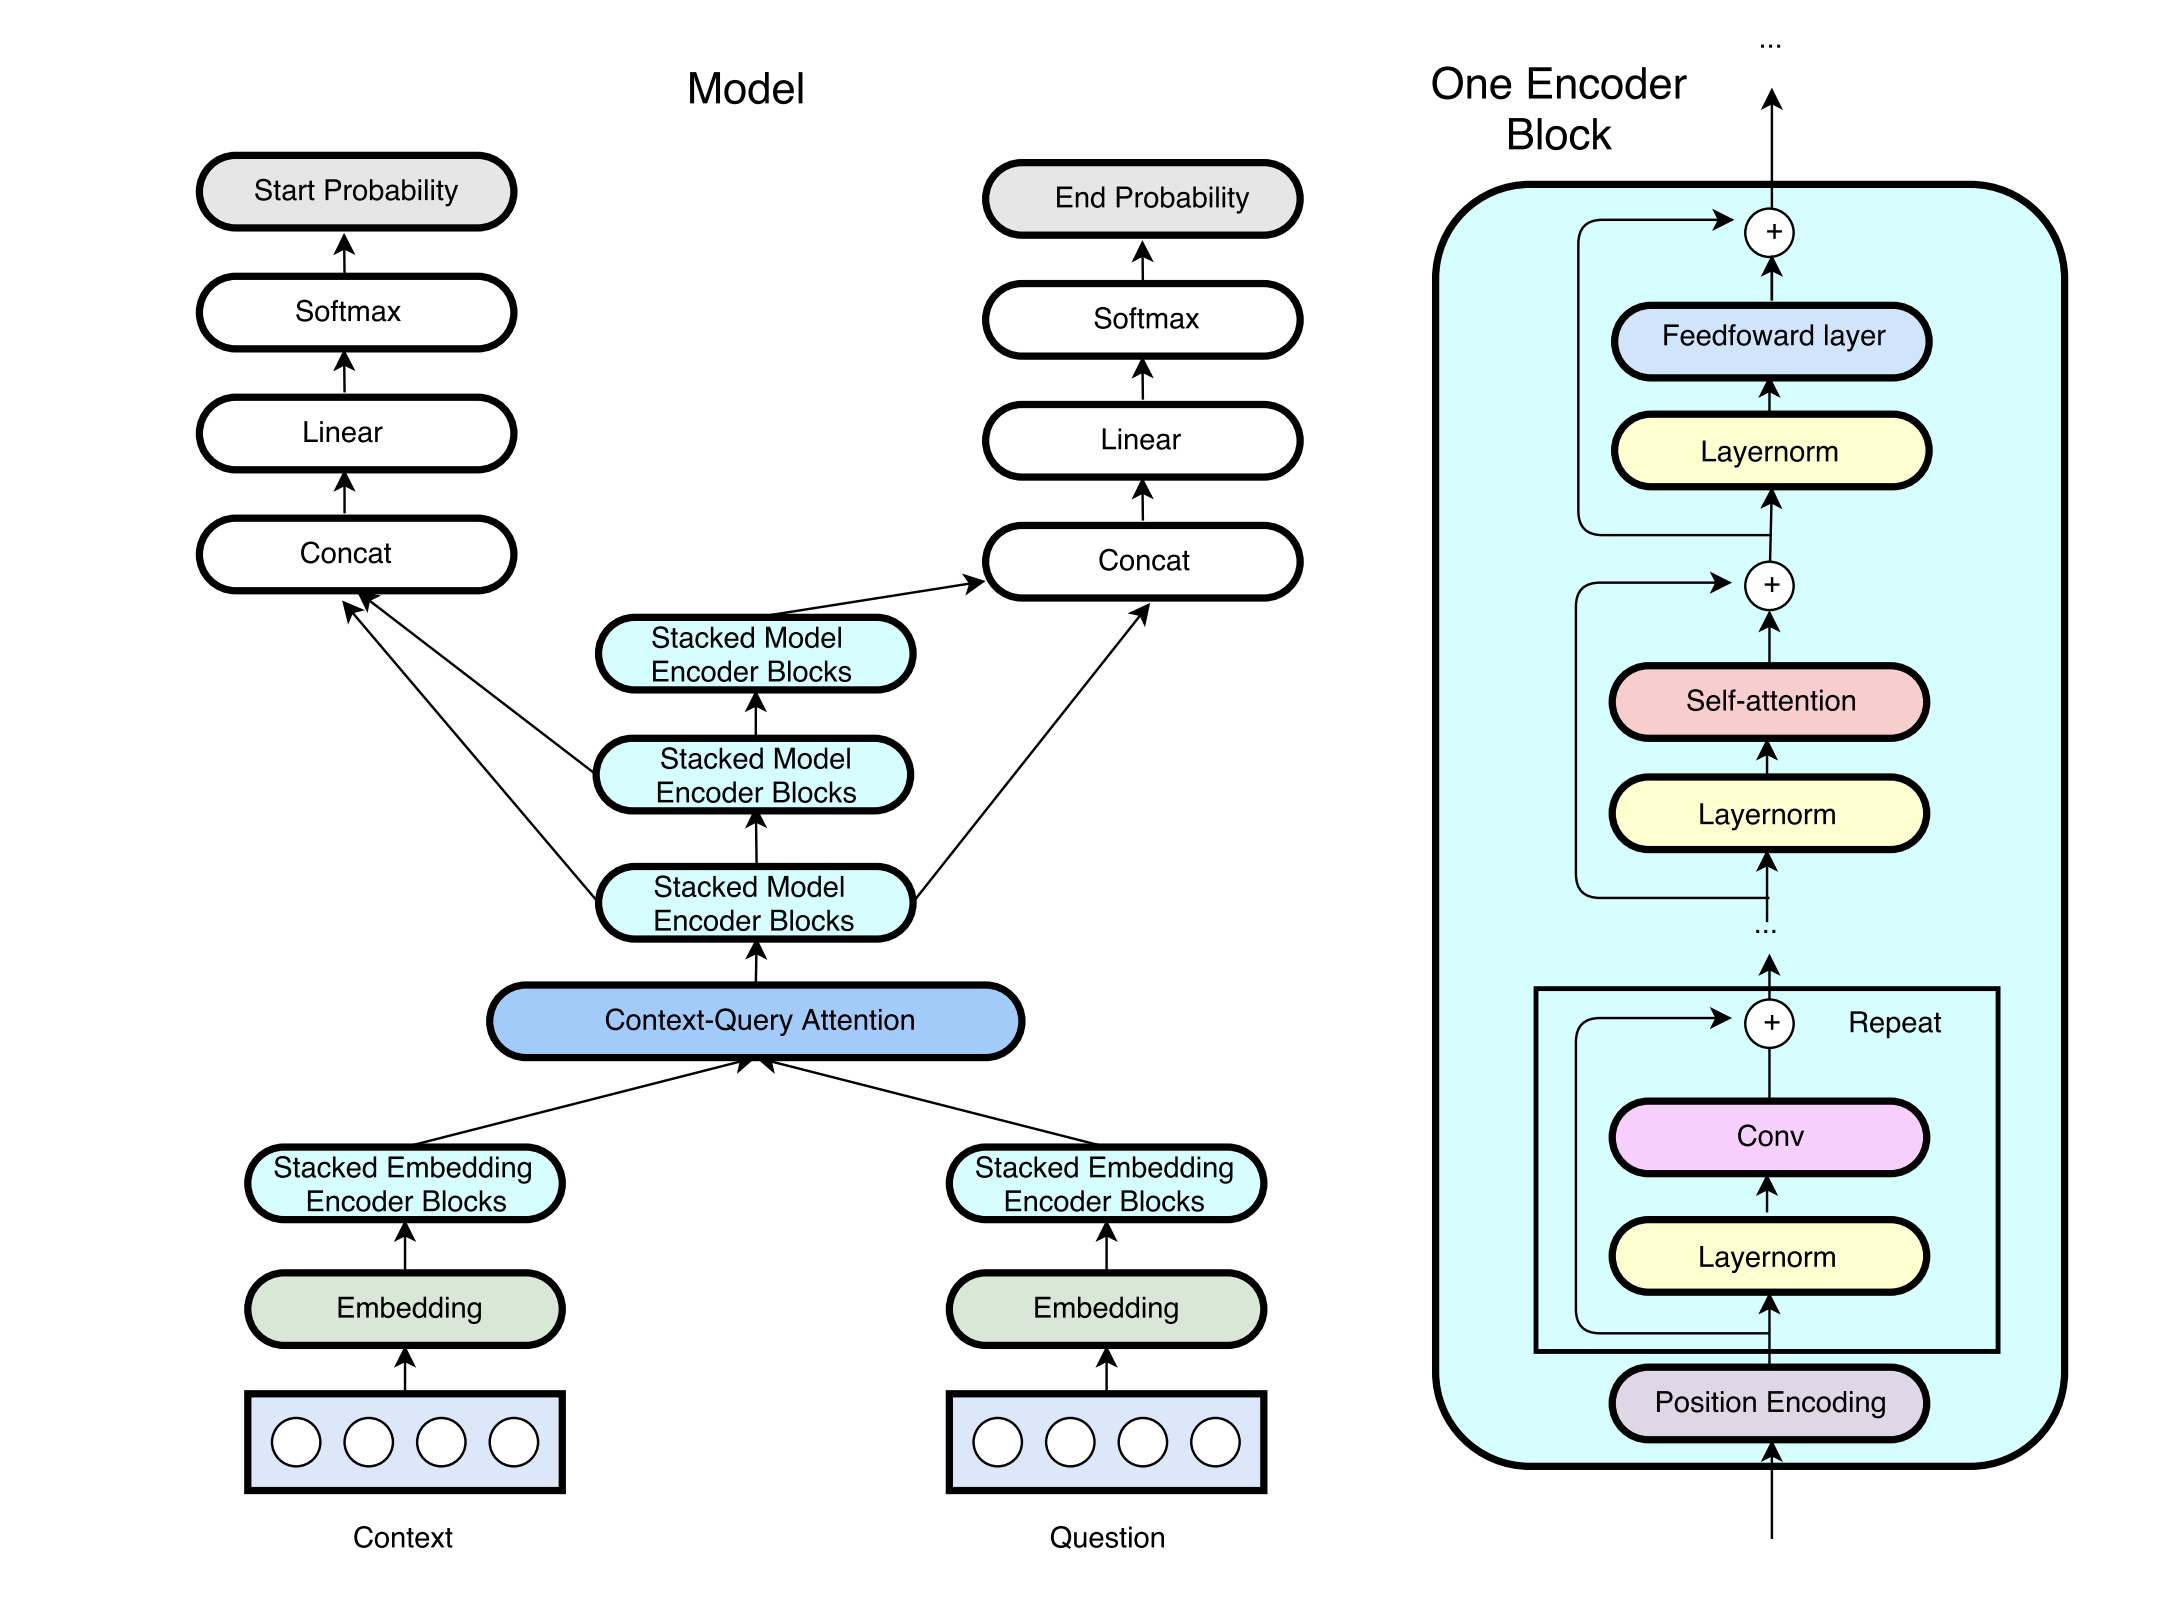
\includegraphics[scale=0.23]{model_diagram}
\caption{Left: Architecture of QANet with convolution and self-attention. Right: Encoder block that is used throughout the model.}
\end{figure}

\subsection{QANet}
We have implemented a version of the QANet model based on the original paper \cite{YU}. The model architecture is summarized in Figure 1. Words are embedded using (1) GLoVE (300-dimensional), and (2) max-pooling of character embeddings (64-dimensional, as provided). In (2), words are truncated/padded to be length 16 and we don't use a convolutional layer as opposed to the approach in the BiDAF implementation \cite{SEO}. These two resulting embeddings are concatenated to form a 364-dimensional embedding for each word. We then project these word representations back to 100 dimensions and pass them through a 2-layer highway network. This is done separately for context words and question words. 

The encoder block of our model consists of the following: a position-encoding \cite{VAS}, a specified number of depthwise-separable 1-dimensional convolutional layers with kernel size 7 and filter size 128 \cite{CHO}, a self-attention layer with 8 heads, and finally a feedforward layer. The self-attention layer is taken from our implementation of this layer in homework 5. Each of these layers except position-encoding is preceded by a layer-norm operation. Residual operation is performed for each layer-norm and its following layer \cite{YU}. \\

Stacked encoder blocks form the embedding encoder layer and the model encoding layer. Word embeddings obtained from the embedding are passed through the embedding encoder layer. This layer has one encoder block which contains 4 convolutional layers. 

The output of the embedding encoder layer is then passed through a context-query attention layer. This is the same attention layer in BiDAF \cite{SEO}. Instead of re-implementing this layer, we use the one in the starter code.

Following this is the model encoder layer. This layer consists of one encoder block used multiple times. The output from the context-query attention layer is fed through the same encoder layer for three times. This encoder block has 2 convolutional layers. All other parameters are set to be the same as those of the encoder blocks in the embedding encoder layer.

The output layer calculates, for each word in the context, the probabilities that (1) it is the start, or (2) the end, of the answer-containing span. This is done by computing 
$$p_{\text{start}}(i)=\text{softmax}(W_1[M_0;M_1]),\;\;\;\; p_{\text{end}}(i)=\text{softmax}(W_2[M_0;M_2]),$$
where $M_0,M_1,$ and $M_2$ denote the outputs of these blocks respectively, $[\cdot \;; \cdot]$ denotes concatenation, and $W_1,W_2$ are trainable parameters. The softmax function that we use is the masked softmax function provided in the starter code.

\subsection{BiDAF with Character-Level Embedding}
In addition to QANet, we have also modified the original BiDAF model by adding a character-embedding component. In the embedding layer, we let the input character embeddings to pass through a 1-dimensional covolutional layer with max-pooling \cite{SEO}. We have also finished an alternative version of this component by passing character embeddings into a 2-dimensional convolutional layer to add in sentence information. The output the convolutional layer is again passed through a ReLu unit and max-pooled on the word-length direction.   
\subsection{Baseline}
We want to compare various implementations of QANet with the result from BiDAF with character-level embedding. 

\section{Experiments}
\subsection{Data}
We use the default SQuAD dataset and the specified preprocessing methods.

\subsection{Experimental Details}
We have finished developing the models as described in the first section and have successfully made them run on our local machines for a long period time. However, we encountered various problems with CUDA when put our models on Azure. We have solved the initial issue of insufficient CUDA memory by reducing batch size. We have also solved the issue of "expecting CPU tensor but get CUDA tensor" by forcing the layers and tensors in the immediate block of code to be on Cuda. However, we currently face the the CUDA device-side assert triggered error as shown in the Figure 2. For both of our modified BiDAF and QANet model, this issue occurs after we run the training for a period of time. We have attempted to solve the issue by changing the version of packages specified in the environment file and by reinstalling relevant packages. Unfortunately, as for now, we are not able to get results for our first leader-board submission.  

\begin{figure}[h]
\centering
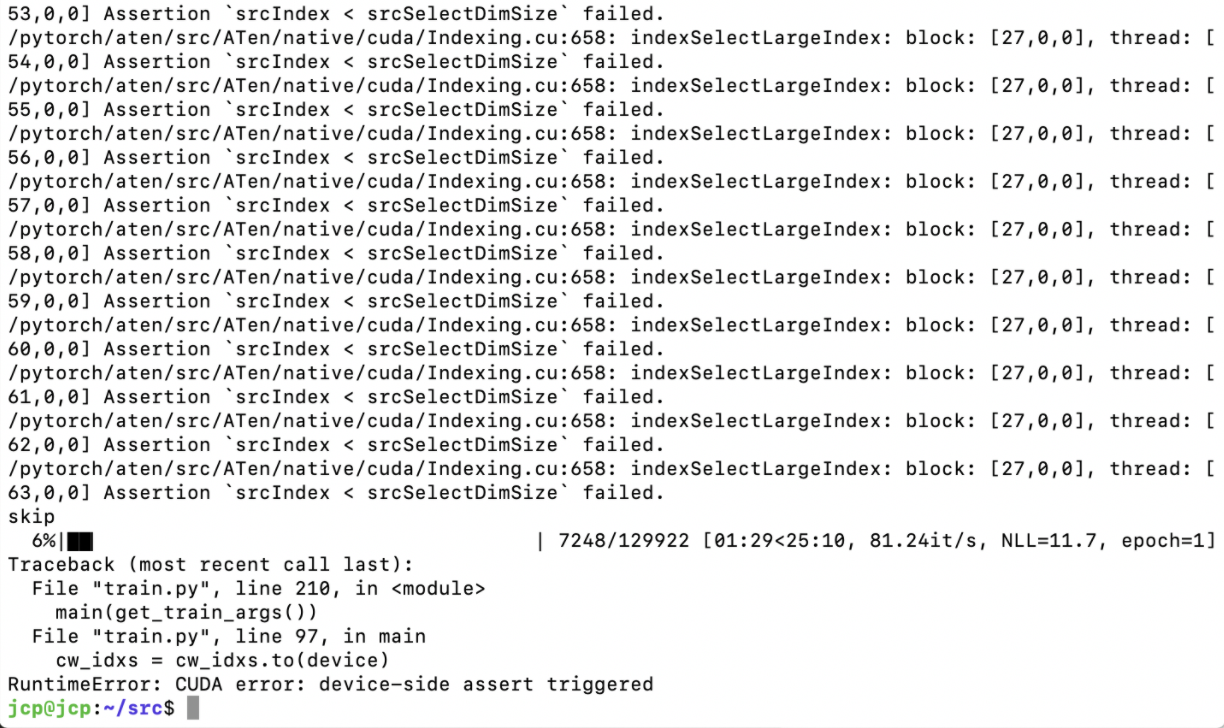
\includegraphics[scale=0.5]{bug}
\caption{The bug that we currently encounter during the training.}
\end{figure}

\subsection{Evaluation}
We plan to use standard exact-match (EM) and F1 scores and examine the behavior of the model when it processes adversarial context.  



\section{Future Work}
For future work, we will solve the training bug and implement the backtranslation data-augmentation technique described in the QANet paper in order to significantly increase the size of our training set.

\bibliographystyle{unsrt}
\bibliography{references}

\end{document}












